
\documentclass[multi,crop,tikz,border=0pt,12pt]{standalone}

\usepackage{latexsym,mathtools}
\def\lineThickness{.7}
\usetikzlibrary{decorations.pathmorphing,shapes}

\definecolor{lightblue}{rgb}{0.8,0.8,1.0}


\begin{document}


%Bruhat poset
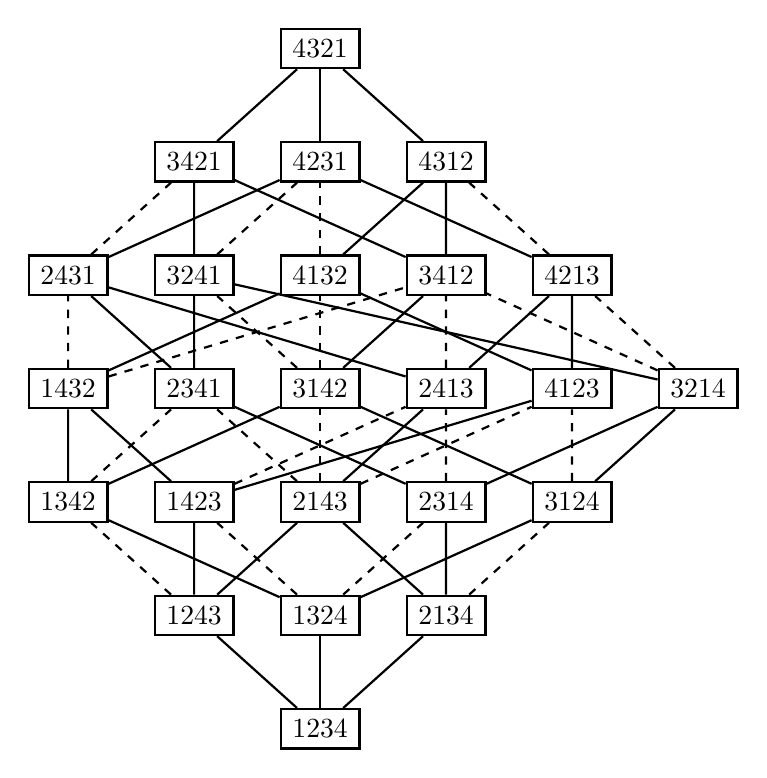
\begin{tikzpicture}[thick,scale=0.4,yscale=-0.9,
every node/.style = {
shape= rectangle,
draw,                    %% here
minimum width  = 1cm,
minimum height = 0.5cm,
align          = center,
text           = black},
black edge/.style  = { -,
thick,
black,
shorten >= 4pt}
]
\node (n1234) at (0.,24.) {1234};
\node (n1243) at (-4.,20.) {1243};
\node (n1324) at (0.,20.) {1324};
\node (n1342) at (-8.,16.) {1342};
\node (n1423) at (-4.,16.) {1423};
\node (n1432) at (-8.,12.) {1432};
\node (n2134) at (4.,20.) {2134};
\node (n2143) at (0.,16.) {2143};
\node (n2314) at (4.,16.) {2314};
\node (n2341) at (-4.,12.) {2341};
\node (n2413) at (4.,12.) {2413};
\node (n2431) at (-8.,8.) {2431};
\node (n3124) at (8.,16.) {3124};
\node (n3142) at (0.,12.) {3142};
\node (n3214) at (12.,12.) {3214};
\node (n3241) at (-4.,8.) {3241};
\node (n3412) at (4.,8.) {3412};
\node (n3421) at (-4.,4.) {3421};
\node (n4123) at (8.,12.) {4123};
\node (n4132) at (0.,8.) {4132};
\node (n4213) at (8.,8.) {4213};
\node (n4231) at (0.,4.) {4231};
\node (n4312) at (4.,4.) {4312};
\node (n4321) at (0.,0.) {4321};
%
\draw(n1234)-- (n1243);
\draw(n1234)-- (n1324);
\draw(n1234)-- (n2134);
\draw[dashed] (n1243)-- (n1342);
\draw(n1243)-- (n1423);
\draw(n1243)-- (n2143);
\draw(n1324)-- (n1342);
\draw[dashed] (n1324)-- (n1423);
\draw[dashed] (n1324)-- (n2314);
\draw(n1324)-- (n3124);
\draw(n1342)-- (n1432);
\draw[dashed] (n1342)-- (n2341);
\draw(n1342)-- (n3142);
\draw(n1423)-- (n1432);
\draw[dashed] (n1423)-- (n2413);
\draw(n1423)-- (n4123);
\draw[dashed] (n1432)-- (n2431);
\draw[dashed] (n1432)-- (n3412);
\draw(n1432)-- (n4132);
\draw(n2134)-- (n2143);
\draw(n2134)-- (n2314);
\draw[dashed] (n2134)-- (n3124);
\draw[dashed] (n2143)-- (n2341);
\draw(n2143)-- (n2413);
\draw[dashed] (n2143)-- (n3142);
\draw[dashed] (n2143)-- (n4123);
\draw(n2314)-- (n2341);
\draw[dashed] (n2314)-- (n2413);
\draw(n2314)-- (n3214);
\draw(n2341)-- (n2431);
\draw(n2341)-- (n3241);
\draw(n2413)-- (n2431);
\draw[dashed] (n2413)-- (n3412);
\draw(n2413)-- (n4213);
\draw[dashed] (n2431)-- (n3421);
\draw(n2431)-- (n4231);
\draw(n3124)-- (n3142);
\draw(n3124)-- (n3214);
\draw[dashed] (n3124)-- (n4123);
\draw[dashed] (n3142)-- (n3241);
\draw(n3142)-- (n3412);
\draw[dashed] (n3142)-- (n4132);
\draw(n3214)-- (n3241);
\draw[dashed] (n3214)-- (n3412);
\draw[dashed] (n3214)-- (n4213);
\draw(n3241)-- (n3421);
\draw[dashed] (n3241)-- (n4231);
\draw(n3412)-- (n3421);
\draw(n3412)-- (n4312);
\draw(n3421)-- (n4321);
\draw(n4123)-- (n4132);
\draw(n4123)-- (n4213);
\draw[dashed] (n4132)-- (n4231);
\draw(n4132)-- (n4312);
\draw(n4213)-- (n4231);
\draw[dashed] (n4213)-- (n4312);
\draw(n4231)-- (n4321);
\draw(n4312)-- (n4321);
%
\end{tikzpicture}

\end{document}
